\newpage
\section{Revisão Bibliográfica e Contexto Tecnológico}
\label{sec:revisao}

Esta revisão organiza-se em três blocos. O primeiro (Seções~\ref{sec:contexto}
e~\ref{sec:quimicas}) examina o contexto de mercado e as químicas de bateria
relevantes para a frota brasileira. O segundo (Seção~\ref{sec:manufatura})
descreve a cadeia de fabricação de células, base do estudo industrial do
Capítulo~\ref{sec:gigafabrica}. O terceiro (Seção~\ref{sec:reciclagem}) revisa
as rotas de reciclagem, a segunda vida e o panorama regulatório, que fundamentam
a discussão das implicações para a cadeia nacional de reciclagem.

% ===========================================================
\subsection{Contexto Energético Global e Nacional}
\label{sec:contexto}
% ===========================================================

\subsubsection{Demanda, Supercapacidade e Custos}
\label{subsec:escala-global}

Segundo a McKinsey \cite{McKinsey2026}, a demanda global por baterias de
íon-lítio, que ultrapassou \textbf{1{,}0~TWh} em 2024, deveria atingir
\textbf{1{,}6~TWh} em 2025. O crescimento apoia-se em dois pilares: a
eletrificação do transporte, maior consumidor de baterias, e o armazenamento
estacionário (BESS), segmento de maior crescimento relativo, essencial para
integrar fontes renováveis intermitentes à rede. A
Figura~\ref{fig:demanda-global-baterias} ilustra a evolução histórica e
projetada por segmento. A série de transporte da figura indica cerca de
2{,}2~TWh em 2030, abaixo do patamar superior a 3{,}0~TWh anuais citado para o
cenário \textit{Stated Policies} da Agência Internacional de Energia
\cite{IEA2025}, diferença que reflete as fontes e os cenários adotados
\pendente{identificar a fonte de cada série da Figura~\ref{fig:demanda-global-baterias}}.

\begin{figure}[H]
\centering
\begin{tikzpicture}
\begin{axis}[
    width  = 15.5cm,
    height = 7.8cm,
    ybar stacked,
    bar width = 11pt,
    xtick          = {0,1,2,3,4,5,6,7,8,9,10,11,12,13,14,15},
    xticklabels    = {2020,2021,2022,2023,2024,2025,2026,2027,2028,
                      2029,2030,2031,2032,2033,2034,2035},
    x tick label style = {rotate=45, anchor=east, font=\footnotesize},
    xmin = -0.7, xmax = 15.7,
    ymin = 0, ymax = 6.3,
    ylabel         = {Demanda global (TWh)},
    ylabel style   = {font=\footnotesize},
    ytick          = {0,1,2,3,4,5,6},
    yticklabel     = {\pgfmathprintnumber[fixed,precision=1]{\tick}},
    yticklabel style = {font=\footnotesize},
    ymajorgrids    = true,
    grid style     = {dotted, gray!35},
    axis line style = {gray!60, line width=0.5pt},
    axis x line*    = bottom,
    axis y line*    = left,
    legend style = {
        at                = {(0.5,-0.34)},
        anchor            = north,
        font              = \footnotesize,
        draw              = none,
        fill              = none,
        legend columns    = 3,
        column sep        = 12pt,
        legend cell align = left,
    },
    clip = false,
]

\addplot[fill=corTransporte, draw=none] coordinates {
    (0,0.145) (1,0.240) (2,0.395) (3,0.585) (4,0.720) (5,1.100)
    (6,1.380) (7,1.620) (8,1.860) (9,2.050) (10,2.200) (11,2.430)
    (12,2.650) (13,2.860) (14,3.060) (15,3.250)
};
\addlegendentry{Transporte (veículos)}

\addplot[fill=corBESS, draw=none, postaction={pattern=north east lines, pattern color=white!70!corBESS}] coordinates {
    (0,0.018) (1,0.040) (2,0.080) (3,0.135) (4,0.190) (5,0.350)
    (6,0.500) (7,0.650) (8,0.780) (9,0.920) (10,1.060) (11,1.210)
    (12,1.370) (13,1.540) (14,1.710) (15,1.890)
};
\addlegendentry{Armazenamento estacionário (BESS)}

\addplot[fill=corOutros, draw=none] coordinates {
    (0,0.027) (1,0.040) (2,0.055) (3,0.070) (4,0.090) (5,0.150)
    (6,0.190) (7,0.230) (8,0.270) (9,0.320) (10,0.370) (11,0.420)
    (12,0.470) (13,0.520) (14,0.570) (15,0.610)
};
\addlegendentry{Outros (eletrônicos, indústria)}

% Rótulos de total em anos-chave
\node[font=\tiny, text=black!75, anchor=south] at (axis cs: 0,  0.34) {0,19};
\node[font=\tiny, text=black!75, anchor=south] at (axis cs: 5,  1.75) {1,60};
\node[font=\tiny, text=black!75, anchor=south] at (axis cs: 10, 3.78) {3,63};
\node[font=\tiny, text=black!75, anchor=south] at (axis cs: 15, 5.90) {5,75};

% Linha de início das projeções (2026)
\draw[corLinha, dashed, line width=0.9pt, dash pattern=on 4pt off 3pt]
    (axis cs: 5.5, 0) -- (axis cs: 5.5, 6.0);
\draw[-{Latex[length=4pt]}, corLinha, line width=0.7pt]
    (axis cs: 5.6, 5.85) -- (axis cs: 7.0, 5.85);
\node[anchor=west, font=\footnotesize\bfseries, text=corLinha]
    at (axis cs: 5.65, 6.10) {Projetado};

\end{axis}
\end{tikzpicture}

\caption{Demanda global por baterias de íon-lítio por segmento de aplicação
         (2020--2035). Valores a partir de 2026 são projetados.}
\label{fig:demanda-global-baterias}
\fonte{adaptado de \citeonline{McKinsey2026} e \citeonline{IEA2025}.}
\end{figure}

Simultaneamente, o mercado atravessa um período de \textbf{supercapacidade
produtiva}, concentrada na Ásia: em 2025, a oferta instalada excedeu a demanda em
aproximadamente 900~GWh, e o custo médio dos pacotes atingiu a mínima histórica de
\textbf{US\$~108/kWh}, redução superior a 50\% em relação a 2018
\cite{McKinsey2026}. Projeções baseadas na \textit{Lei de Wright} — que relaciona
a redução de custos ao volume acumulado de produção — indicam que os pacotes
LFP/LMFP podem chegar a \textbf{US\$~55 a 65/kWh até 2035}, assumindo preços
estáveis de matérias-primas e ganhos de eficiência em processos como o
revestimento de eletrodos a seco (\textit{dry coating}) \cite{EUROBAT}.

A queda de preços tem duplo efeito. De um lado, acelera a paridade de custo total
de propriedade (\textit{Total Cost of Ownership} — TCO) entre veículos elétricos
e a combustão, inclusive em mercados emergentes como o Brasil; de outro, reduz o
valor relativo dos materiais recuperados pela reciclagem, sobretudo nas químicas
de menor valor intrínseco, como a LFP (Seção~\ref{subsec:lfp-economics}). A
pressão sobre as cadeias de lítio, níquel e cobalto — minerais de distribuição
geográfica concentrada e mercados instáveis — impulsiona ainda a diversificação
das químicas: a migração do NMC para o LFP em segmentos de volume, o surgimento
do LMFP, o desenvolvimento do sódio-íon e a entrada gradual das baterias em
estado sólido (Seção~\ref{sec:quimicas}).

\subsubsection{O Contexto Energético Brasileiro}
\label{subsec:contexto-brasil}

O Brasil ocupa uma posição particular na transição para a mobilidade elétrica,
condicionada por três fatores estruturais que moldam o perfil de sua frota
eletrificada e, consequentemente, o fluxo de materiais de baterias.

\paragraph{A rota híbrida flex como caminho próprio.}
Enquanto a Europa e a China priorizam veículos puramente elétricos (BEV) e
híbridos \textit{plug-in}, a frota nacional sinaliza uma preferência por
veículos urbanos de baixo custo e por rotas híbridas — em particular os
Híbridos-Flex (HEV Flex) e os Híbridos \textit{Plug-in} (PHEV). Essa preferência
decorre da ampla disponibilidade de etanol e da vasta infraestrutura de postos de
combustível. Nesse contexto, os Veículos Elétricos com Extensor de Autonomia
(REEV — \textit{Range Extended Electric Vehicle}) surgem como alternativa
promissora, pois operam primariamente em modo elétrico e utilizam o etanol como
fonte secundária de energia \cite{BrightConsulting}.

\paragraph{A predominância de modelos asiáticos de entrada.}
A expansão da mobilidade elétrica no Brasil é tracionada majoritariamente por
montadoras asiáticas — especialmente BYD, GWM e JAC —, que priorizam as químicas
LFP e NMC para reduzir o preço final ao consumidor em um mercado sensível a
custo. A composição química resultante na amostra analisada neste trabalho é
apresentada na Seção~\ref{sec:marketshare}.

\paragraph{A implicação direta para o fluxo de materiais.}
As baterias de híbridos convencionais são significativamente menores do que as
de veículos puramente elétricos: um HEV típico opera com um pacote de 1 a 2~kWh,
enquanto um BEV popular carrega entre 30 e 80~kWh. A demanda por lítio e demais
minerais críticos por veículo é, portanto, menor no cenário brasileiro do que
seria em uma eletrificação plena baseada em BEV. Essa vantagem por unidade não
elimina a necessidade de uma infraestrutura de reciclagem e logística reversa,
uma vez que o volume acumulado de baterias em fim de vida crescerá de forma
contínua ao longo das próximas décadas \cite{EPE2025,MBCBrasil}. A
Tabela~\ref{tab:comparativo-mercados} sintetiza as diferenças entre a trajetória
brasileira e as dos principais mercados de referência.

\begin{table}[H]
    \centering
    \caption{Comparativo da trajetória de eletrificação: Brasil vs.\ mercados
             globais de referência.}
    \label{tab:comparativo-mercados}
    \renewcommand{\arraystretch}{1.4}
    \small
    \rowcolors{2}{gray!10}{white}
    \begin{tabularx}{\textwidth}{
        >{\raggedright\arraybackslash}p{3.6cm}
        >{\raggedright\arraybackslash}X
        >{\raggedright\arraybackslash}X
        >{\raggedright\arraybackslash}X }
    \toprule
    \textbf{Dimensão} & \textbf{Brasil} & \textbf{Europa} & \textbf{China} \\
    \midrule
    Tecnologia dominante & Híbrido-Flex (HEV) e PHEV & BEV de longo alcance & BEV e PHEV \\
    Química predominante & LFP, seguido de NMC e NiMH (Seção~\ref{sec:marketshare}) & NMC (45\%+) & LFP ($>$55\%) \\
    Combustível alternativo & Etanol (flex) & -- & -- \\
    Horizonte de 30\% da frota eletrificada & $\sim$2040 & $\sim$2030 & Já superado em regiões-chave \\
    Principal indutor & Programas Mover e Novo PAC & Regulação de CO$_2$ e fim dos ICE & Subsídios diretos e mandatos \\
    \bottomrule
    \end{tabularx}
    \fonte{elaborada pelos autores \pendente{indicar as fontes dos valores de Europa e China}.}
\end{table}

% ===========================================================
\subsection{Química das Baterias}
\label{sec:quimicas}
% ===========================================================

A escolha da química de bateria determina a densidade energética disponível por
veículo, o custo por kWh, os riscos da cadeia de suprimentos e, sobretudo, a
composição dos materiais que futuramente entrarão no fluxo de reciclagem. Esta
seção revisa as químicas presentes na frota brasileira — NMC, LFP/LMFP e NiMH —
e, de forma resumida, as tecnologias emergentes de sódio-íon e estado sólido.

\subsubsection{NMC (Níquel-Manganês-Cobalto)}
\label{subsec:nmc}

As baterias NMC consolidaram-se como o padrão de alto desempenho para veículos de
longo alcance e segmentos \textit{premium}, pela elevada densidade energética. A
família é caracterizada pela proporção de níquel, manganês e cobalto no cátodo; ao
longo da última década, a indústria migrou da composição original NMC~111 (um
terço de cada metal) para as variantes NMC~532 e NMC~622 e, depois, para o
NMC~811 (80\% Ni, 10\% Mn e 10\% Co), de maior densidade energética e maior
sensibilidade térmica, com o NMC de alto manganês como direção futura.

A dependência de cobalto e níquel expõe o NMC à volatilidade de preços e a riscos
geopolíticos: a República Democrática do Congo responde por mais de 70\% da
produção mundial de cobalto \cite{IEA2025}, e o níquel de alta pureza é
majoritariamente produzido na Indonésia e nas Filipinas. Projeta-se que o NMC
represente entre 43\% e 45\% da demanda na União Europeia e na América do Norte
até 2035 \cite{McKinsey2026}. No Brasil, sensível a preço, a química tende a
ocupar um nicho — veículos de alta performance, PHEVs de categorias superiores e
frotas de longo curso —, embora seja a segunda mais frequente na amostra
analisada, com presença expressiva em modelos da GWM, Volvo e CAOA Chery
(Seção~\ref{sec:marketshare}).

\subsubsection{LFP e a Transição para LMFP}
\label{subsec:lfp}

A consolidação do Lítio-Ferro-Fosfato (LFP) como química predominante para
veículos de entrada e de volume é um dos fenômenos mais marcantes da década: em
2024, as baterias LFP já representavam quase 50\% do mercado global de veículos
elétricos \cite{McKinsey2026}, impulsionadas por segurança intrínseca superior,
vida útil mais longa e custo de produção muito inferior ao das químicas baseadas
em níquel e cobalto.

A estrutura cristalina do LFP confere estabilidade térmica excepcional: ao
contrário do NMC, o LFP não libera oxigênio em condições de abuso térmico, o que
reduz drasticamente o risco de \textit{thermal runaway}, simplifica o sistema de
gerenciamento térmico do pacote e reduz seu custo. Em contrapartida, o potencial
nominal da célula LFP ($\approx$3,2~V) é inferior ao do NMC ($\approx$3,6--3,7~V),
o que resulta em menor densidade energética e exige pacotes maiores e mais pesados
para autonomias equivalentes.

O LMFP (Lítio-Manganês-Ferro-Fosfato) surge como evolução natural da Geração~3:
a substituição parcial do ferro pelo manganês eleva o potencial de operação de
aproximadamente 3,2~V para 3,7--4,0~V, com ganho de densidade energética de 15\%
a 20\% em relação ao LFP convencional \cite{EUROBAT}. A competitividade das
químicas de ferro deve intensificar-se em três fases: adoção em massa do LMFP em
veículos leves (2025--2028); domínio de mercado, com participação conjunta de LFP
e LMFP entre 49\% e 52\% na Europa e na América do Norte até 2035
\cite{McKinsey2026}; e aproximação do piso de custo discutido na
Seção~\ref{subsec:escala-global}.

Para o mercado brasileiro, a força do LFP/LMFP é ainda mais pronunciada — trata-se
da química mais frequente na amostra analisada (Seção~\ref{sec:marketshare}).
Essa predominância impõe um desafio à cadeia de reciclagem: ao contrário do NMC,
cujo cobalto e níquel têm elevado valor de mercado, os componentes do LFP (ferro,
fósforo e lítio em menor concentração) têm valor comercial significativamente
menor por tonelada, o que dificulta a viabilidade econômica da recuperação sem
ganhos expressivos de escala — efeito amplificado pela queda contínua dos preços
de baterias novas.

\subsubsection{NiMH (Níquel-Metal Hidreto)}
\label{subsec:nimh}

As baterias NiMH tiveram papel fundacional na eletrificação automotiva como
principal tecnologia dos híbridos convencionais (HEV), desde a década de 1990.
Oferecem alta densidade de potência — fundamental para capturar a energia de
frenagem regenerativa e fornecer picos de potência —, confiabilidade operacional
comprovada, inclusive em clima tropical, e segurança térmica superior
\cite{McKinsey2026}. A menor densidade energética restringe seu uso a sistemas
em que a bateria atua de forma auxiliar ao motor a combustão.

No Brasil, impulsionado pela rota dos híbridos-flex, o NiMH é a terceira química
mais frequente na amostra analisada (Seção~\ref{sec:marketshare}). Sob a ótica do
fluxo de materiais, apresenta dinâmica oposta à do LFP: composto por proporções
significativas de \textbf{níquel} e de \textbf{elementos de terras raras} —
lantânio, cério e neodímio — no eletrodo negativo, tem elevado valor intrínseco
de reciclagem, o que favorece a viabilidade da logística reversa. Mesmo com a
migração gradual para soluções baseadas em lítio, o volume acumulado de baterias
NiMH no país permanecerá representativo.

\subsubsection{Tecnologias Emergentes: Sódio-Íon e Estado Sólido}
\label{subsec:naion}
\label{subsec:estadosolido}

As baterias de \textbf{sódio-íon} apoiam-se na abundância geográfica do sódio e na
compatibilidade com a infraestrutura de fabricação existente para o lítio.
Permitem o uso de coletores de alumínio nos dois eletrodos — dispensando o cobre —
e o armazenamento e transporte com tensão zero, o que aumenta a segurança
logística \cite{McKinsey2026}. A menor densidade energética resulta em maior
intensidade de materiais por kWh, e a viabilidade em veículos leves depende de
avanços como ânodos de carbono duro acima de 400~mAh/g e tensões de operação de
4,2~V. Em mercados estáveis, a paridade de preço com o LFP só deve ser alcançada
em meados de 2035; em caso de choques no suprimento de grafite ou lítio, a
paridade pode ocorrer já em 2032 \cite{McKinsey2026}. Os nichos esperados são
veículos compactos de entrada, micro-carros, sistemas auxiliares de 12~V e
armazenamento estacionário de curta duração; para o Brasil, o sódio-íon tende a
complementar, e não substituir, a rota baseada em LFP.

As baterias em \textbf{estado sólido} substituem o eletrólito líquido por um
condutor sólido. Na escala TRL adotada pela EUROBAT, encontram-se majoritariamente
entre os níveis 4 e 6 em 2025, com exceção das células de semi-estado sólido
(TRL 7--8). As projeções indicam densidades de 400 a 450~Wh/kg até 2030, recarga
completa em 12 a 20~minutos, custo em torno de US\$~100/kWh e vida útil de 1.000 a
1.500 ciclos \cite{McKinsey2026}. Gargalos de manufatura — interfaces homogêneas
entre camadas sólidas e baixo rendimento de produção — devem restringir a
tecnologia a nichos de alto valor no curto prazo; no horizonte deste trabalho
(até 2040), ela não figura como fator relevante no fluxo de materiais da frota
brasileira.

\subsubsection{Comparação entre as Tecnologias}
\label{sec:comparacao}

A Figura~\ref{fig:intensidade-materiais} apresenta a intensidade de materiais por
kWh de cada tecnologia, e a Tabela~\ref{tab:comparativo-quimicas} sintetiza suas
dimensões técnicas, econômicas e ambientais. Para o LFP, os valores da figura
diferem da composição de célula adotada no Capítulo~\ref{sec:gigafabrica} —
por exemplo, cerca de 0,5~kg de grafite e 0,25~kg de alumínio, cobre e
eletrólito somados por kWh na figura, contra 1,17~kg de grafite
(Tabela~\ref{tab:giga-anodo}) e cerca de 2,5~kg desses três componentes,
incluído o invólucro de alumínio (Tabela~\ref{tab:giga-balanco-celula}) —, o
que indica bases distintas
\pendente{declarar a base da Figura~\ref{fig:intensidade-materiais}: célula ou
pacote; massa de elemento ou de composto}.

\begin{figure}[H]
    \centering
    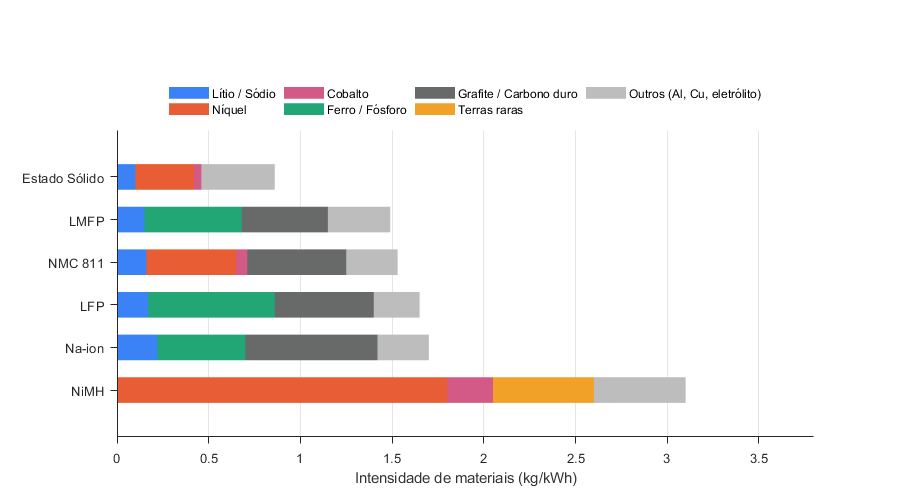
\includegraphics[width=\textwidth]{figuras/comparacao_quimica_baterias.png}
    \caption{Intensidade de materiais por tecnologia de bateria (kg por kWh).}
    \label{fig:intensidade-materiais}
    \fonte{elaborada com base em \citeonline{IEA2025} e \citeonline{McKinsey2026}.}
\end{figure}

\begin{table}[H]
\centering
\caption{Comparativo entre as tecnologias de bateria relevantes para a frota
         eletrificada brasileira.}
\label{tab:comparativo-quimicas}
\renewcommand{\arraystretch}{1.4}
\small
\begin{tabularx}{\textwidth}{@{} p{2.2cm} X X X @{}}
\toprule
\textbf{Tecnologia} & \textbf{Aspectos técnicos} &
\textbf{Dimensão econômica} & \textbf{Implicações para o fluxo de materiais} \\
\midrule
\textbf{NMC} &
Alta densidade energética; ideal para veículos de longa distância e
\textit{premium}. &
Custo elevado e volátil devido ao Co e ao Ni; foco em mercados maduros (UE/EUA). &
Alta dependência de minerais críticos com cadeias de suprimento instáveis; alto
valor de reciclagem. \\
\addlinespace
\textbf{LFP / LMFP} &
Alta segurança e longa vida útil; a evolução LMFP aumenta a densidade em até 20\%. &
Líder em custo-benefício (alvo de US\$~55--65/kWh); base da eletrificação de massa
no Brasil. &
Desafio na reciclagem: baixo valor dos materiais (Fe, P) dificulta a viabilidade
econômica sem escala. \\
\addlinespace
\textbf{NiMH} &
Alta densidade de potência e confiabilidade; limitada por menor densidade
energética; ideal para HEV. &
Tecnologia madura com custo consolidado; forte presença no Brasil via
híbridos-flex de alto volume. &
Elevado valor de reciclagem (Ni e terras raras); logística reversa economicamente
viável. \\
\addlinespace
\textbf{Na-ion} &
Menor densidade que o lítio; permite armazenamento com tensão zero, aumentando a
segurança logística. &
Tecnologia de reserva (\textit{backstop}) contra a volatilidade do lítio; paridade
de preço prevista para 2035. &
Abundância geográfica do sódio; reduz dependência de minerais escassos e o uso de
cobre. \\
\addlinespace
\textbf{Estado sólido} &
Fronteira tecnológica: densidade disruptiva (400+ Wh/kg) e recarga ultra-rápida
(12--20~min). &
Nicho de alto valor inicial; escala comercial projetada apenas para pós-2030 a
$\sim$US\$~100/kWh. &
Promete maior durabilidade (1.000--1.500 ciclos); fluxo de resíduos irrelevante no
horizonte desta pesquisa. \\
\bottomrule
\end{tabularx}
\fonte{elaborada pelos autores com base nas Seções~\ref{subsec:nmc} a~\ref{subsec:estadosolido}.}
\end{table}

% ===========================================================
\subsection{Manufatura de Células de Íon-Lítio}
\label{sec:manufatura}
% ===========================================================

A fabricação de células de íon-lítio organiza-se em três blocos de processo
\cite{knehr2022batpac,degen2022}: (i)~a produção de eletrodos — mistura dos
materiais ativos, aditivos condutores e aglutinantes em pasta, revestimento sobre
as folhas coletoras (alumínio no catodo, cobre no anodo), secagem com recuperação
do solvente e calandragem; (ii)~a montagem da célula — corte, empilhamento ou
enrolamento com o separador, inserção no invólucro e soldagem, em sala seca de
baixo ponto de orvalho, seguidas do enchimento com eletrólito e da selagem; e
(iii)~o acabamento — formação da interface sólido-eletrólito (SEI) por ciclos de
carga controlados, degasagem, envelhecimento e teste para classificação das
células.

Dois aspectos dessa cadeia são centrais para a análise de fluxos. O primeiro é a
geração de refugo em todas as etapas — pasta fora de especificação na mistura,
eletrodo revestido descartado no revestimento e no corte e células reprovadas na
formação e no teste —, de composição conhecida e homogênea, o que o diferencia das
baterias pós-consumo (Seção~\ref{subsec:lfp-economics}). O segundo é a
concentração do consumo de energia em operações que não transformam
quimicamente o material: a secagem dos eletrodos com recuperação do solvente
N-metil-2-pirrolidona (NMP), o controle de umidade da sala seca e a formação
respondem pela maior parte da energia da planta \cite{degen2022}. O
Capítulo~\ref{sec:gigafabrica} quantifica esses fluxos para uma fábrica de células
LFP.

% ===========================================================
\subsection{Reciclagem, Segunda Vida e Regulação}
\label{sec:reciclagem}
% ===========================================================

À medida que a frota eletrificada brasileira se expande, o destino das baterias ao
fim de sua vida útil torna-se mais urgente. A reciclagem de baterias de íon-lítio
(LIB) cumpre um papel duplo: resposta ambiental necessária para evitar a
contaminação por metais pesados e oportunidade estratégica de recuperação de
materiais críticos — lítio, cobalto, níquel e manganês — que realimentam a
produção de novas células. Esta seção apresenta as tecnologias de reciclagem,
analisa os desafios econômicos da química LFP, discute a segunda vida e
contextualiza o panorama regulatório.

\subsubsection{Pré-tratamento e Preparação das Células}
\label{subsec:pretratamento}

Independentemente da rota, as tecnologias de recuperação compartilham etapas de
pré-tratamento que determinam a eficiência, a segurança e o custo das fases
subsequentes \cite{latini2022apudhu2024}. A primeira é a descarga elétrica das
células, que devem ser reduzidas a uma tensão inferior a 1{,}5\,V antes de
qualquer manipulação mecânica. Na sequência, a trituração (\textit{shredding}), o
peneiramento e a separação por densidade produzem a \textit{black mass} —
mistura dos materiais ativos do catodo e do anodo com impurezas —, insumo central
das etapas piro e hidrometalúrgicas, cuja qualidade influencia diretamente a
eficiência da recuperação.

A logística reversa que antecede o pré-tratamento é ela própria um gargalo: em
revisão de 60 estudos, \citeonline{slattery2021} identificaram a coleta e o
transporte como desafio à reutilização ou à reciclagem em 70\% deles, e o
transporte respondeu, em média, por cerca de 41\% do custo total de reciclagem
nos estudos de custo analisados.

\subsubsection{Rotas de Reciclagem}
\label{subsec:rotas}

A literatura consolida cinco grandes rotas tecnológicas para a reciclagem de LIBs
\cite{biswal2024,balachandran2024}: pirometalurgia, hidrometalurgia, reciclagem
direta, biolixiviação e métodos eletroquímicos.

\paragraph{Pirometalurgia.}
Rota mais madura e amplamente implantada comercialmente (TRL~9). Consiste na fusão
das células ou da \textit{black mass} a \textbf{1.400--1.500\,°C}, produzindo uma
liga metálica rica em cobalto, níquel e cobre, posteriormente refinada por etapas
hidrometalúrgicas. Suas limitações incluem a perda de lítio e grafite para a
escória, a alta intensidade energética e a emissão de compostos fluorados da
decomposição do eletrólito (LiPF\textsubscript{6}). Para o LFP — cujo principal
elemento de valor, o lítio, é perdido na escória, e cujos ferro e fósforo têm
baixo valor de recuperação —, a adequação é baixa. Em termos climáticos, a revisão
de \citeonline{stegemann2025} indica que a combinação de rotas piro e
hidrometalúrgicas reduz em 27\% as emissões associadas à produção da célula.

\paragraph{Hidrometalurgia.}
Rota de maior presença na literatura — cerca de 57\% das publicações sobre
reciclagem de LIBs \cite{zhao2025}. Baseia-se na dissolução da \textit{black
mass} em soluções ácidas (clorídrico, sulfúrico ou nítrico), seguida de
purificação, precipitação seletiva e extração por solvente para separar lítio,
cobalto, níquel, manganês e cobre em compostos de alta pureza. Apresenta menor
intensidade energética ($<$100\,°C), recupera o lítio como carbonato ou hidróxido
de grau bateria ($>$90\% em meio ácido) e pode ser dimensionada para volumes
menores, o que a torna mais adequada a mercados emergentes como o Brasil.
\citeonline{stegemann2025} reportam redução de 39\% nas emissões da produção da
célula, com média de $-25{,}5$~kg\,CO\textsubscript{2}eq/kWh entre os estudos de
baterias NMC analisados — o melhor desempenho entre as rotas avaliadas na revisão.
Para o LFP, a viabilidade econômica permanece frágil, dado o baixo valor dos
materiais recuperados (Seção~\ref{subsec:lfp-economics}).

\paragraph{Reciclagem direta (\textit{direct recycling}).}
Visa \textbf{preservar e regenerar a estrutura cristalina} do material ativo do
cátodo, evitando a dissolução e a re-síntese química completa, por meio de
(i)~separação e coleta do material ativo, (ii)~relitiação e (iii)~tratamento
térmico para restaurar a ordem estrutural. O material regenerado pode ser usado
diretamente em novas baterias. \citeonline{balachandran2024} identificam essa rota
como a de maior potencial para a economia circular, mas com desafios de
homogeneidade dos lotes de entrada e de reprodutibilidade do desempenho
eletroquímico. Para o LFP, a estabilidade do LiFePO\textsubscript{4} facilita a
regeneração, e estudos recentes demonstraram a recuperação de
FePO\textsubscript{4} de resíduos de extração de lítio para uso em novas células
\cite{hu2024}. Maturidade atual: TRL~5--7.

\paragraph{Biolixiviação e métodos eletroquímicos.}
A biolixiviação utiliza microrganismos acidofílicos (principalmente
\textit{Acidithiobacillus thiooxidans} e \textit{A.~ferrooxidans}) para solubilizar
metais da \textit{black mass} com menor consumo de reagentes, mas ainda apresenta
taxas de extração mais baixas e tempos de processo mais longos (TRL~3--5)
\cite{balachandran2024}. Os métodos eletroquímicos recuperam seletivamente metais
de soluções de lixiviação, com alta seletividade iônica e compatibilidade com
fontes renováveis; hoje são usados sobretudo como etapas de purificação em fluxos
hidrometalúrgicos, com desenvolvimento industrial pleno projetado para o período
pós-2030 (TRL~4--6) \cite{zhu2024}. A Tabela~\ref{tab:rotas-reciclagem} sintetiza
as rotas.

\begin{table}[H]
\centering
\caption{Comparativo entre as rotas de reciclagem de baterias de íon-lítio.}
\label{tab:rotas-reciclagem}
\small
\renewcommand{\arraystretch}{1.2}
\begin{tabularx}{\textwidth}{@{} p{3cm} X X X X @{}}
\toprule
\textbf{Critério} & \textbf{Pirometalurgia} & \textbf{Hidrometalurgia} &
\textbf{Reciclagem Direta} & \textbf{Bio / Eletroquímica} \\
\midrule
Maturidade (TRL) & Alta (TRL~9) — comercial & Alta (TRL~9) — comercial &
Média (TRL~5--7) — piloto & Baixa/Média (TRL~3--6) — laboratório \\
\addlinespace
Temperatura & 1.400--1.500\,°C & $<$100\,°C & 200--900\,°C (recozimento) &
Ambiente ($\sim$25--50\,°C) \\
\addlinespace
Recuperação de Li & Muito baixa (Li vai para a escória) &
Alta ($>$90\% em meio ácido) & Alta (com relitiação) & Moderada a alta \\
\addlinespace
Adequação ao LFP & Baixa — Li perdido na escória; Fe e P sem valorização &
Moderada — rentabilidade limitada & Alta — estrutura olivínica estável &
Em avaliação \\
\addlinespace
Impacto climático$^{a}$ & $-$27\% (rotas piro e hidro combinadas) &
$-$39\% & Potencialmente inferior ao hidro & Em estudo \\
\addlinespace
Custo relativo & Alto (\textit{capex} elevado, escala de fusão) &
Médio (reagentes + efluentes) & Baixo/Médio (dependente de escala) &
Baixo (perspectiva de longo prazo) \\
\bottomrule
\end{tabularx}
\par\vspace{2pt}{\footnotesize $^{a}$Redução das emissões em relação à produção
da célula \cite{stegemann2025}.}
\fonte{adaptado de \citeonline{balachandran2024} e \citeonline{stegemann2025}.}
\end{table}

\subsubsection{Desafios Econômicos da Reciclagem do LFP}
\label{subsec:lfp-economics}

A predominância de baterias LFP na frota eletrificada brasileira coloca o país
diante de uma dificuldade estrutural de reciclagem. Ao contrário das baterias NMC,
que contêm cobalto e níquel em proporções significativas, os componentes do LFP
(lítio, ferro e fósforo) possuem valor intrínseco substancialmente menor. O valor
de mercado dos materiais recuperados de baterias LFP situa-se entre USD~300 e
USD~600 por tonelada \pendente{indicar a fonte original; o valor não consta de
\citeonline{stegemann2025}}, o que resulta em prejuízo líquido sob as condições
operacionais atuais da maior parte das instalações. Os recicladores tendem a
priorizar materiais críticos de maior valor, e as baterias LFP são menos propensas
a ser recicladas \cite{nrel2023}.

Esse cenário é agravado pela queda do preço do carbonato de lítio — que recuou de
picos históricos em 2022 para valores muito inferiores em 2024--2025 —, que reduz o
incentivo à recuperação do lítio. \citeonline{chen2025} identificam gargalos
adicionais: a estabilidade da estrutura olivínica do LiFePO\textsubscript{4} exige
condições ácidas mais agressivas de lixiviação; o ferro e o fósforo não possuem
rotas de valorização simples nas cadeias existentes; e normas crescentes sobre
efluentes ácidos e resíduos fluorados elevam os custos de conformidade. Somente
grandes volumes reduzem o custo unitário ao ponto de rentabilidade; no Brasil, o
momento em que os volumes de fim de vida atingirão essa escala depende do MFA
dinâmico da frota, indicado como continuidade deste trabalho
(Capítulo~\ref{sec:conclusao}).

A resposta tecnológica mais promissora é a reciclagem direta do material ativo
do catodo LFP, que elimina a dissolução e a re-síntese química completa;
complementarmente, a recuperação de grafite, inclusive a partir de baterias LFP,
pode melhorar a economia do processo \cite{nrel2023}. Nesse contexto, a sucata de
produção — homogênea, de composição conhecida e livre de contaminação — tende a
ser economicamente mais atrativa do que o material pós-consumo e é quantificada
no Capítulo~\ref{sec:gigafabrica}. A Tabela~\ref{tab:lfp-gargalos} sintetiza
esses gargalos.

\begin{table}[H]
\centering
\caption{Gargalos econômicos da reciclagem de baterias LFP e implicações para o
         contexto brasileiro.}
\label{tab:lfp-gargalos}
\small
\renewcommand{\arraystretch}{1.2}
\begin{tabularx}{\textwidth}{@{} p{3cm} X X @{}}
\toprule
\textbf{Fator} & \textbf{Descrição} & \textbf{Implicação para o Brasil} \\
\midrule
Baixo valor intrínseco dos materiais &
Fe e P têm valor de mercado muito inferior ao Co e ao Ni do NMC &
Margens negativas nas operações convencionais; recicladores priorizam
materiais de maior valor \\
\addlinespace
Queda do preço do carbonato de lítio &
Pico histórico em 2022; recuo acentuado em 2024--2025 reduz o valor do Li
recuperado &
Diminui o único componente de valor relativo do LFP, piorando a equação econômica \\
\addlinespace
Dificuldade de lixiviação seletiva &
Estrutura olivínica estável exige condições ácidas mais agressivas, elevando o
custo de reagentes &
Aumenta o custo operacional da hidrometalurgia aplicada ao LFP \\
\addlinespace
Baixa separabilidade de Fe e P &
Ferro e fósforo não possuem rotas de valorização simples nas cadeias existentes &
Limita receitas secundárias e onera o tratamento de efluentes \\
\addlinespace
Escala insuficiente (curto prazo) &
Apenas grandes volumes reduzem o custo unitário ao ponto de rentabilidade &
Momento de atingir escala depende dos volumes de fim de vida da frota (MFA
dinâmico, etapa futura); a sucata de produção pode antecipar parte dessa escala \\
\bottomrule
\end{tabularx}
\fonte{elaborada com base em \citeonline{chen2025} e \citeonline{nrel2023}.}
\end{table}

\subsubsection{Segunda Vida das Baterias (\textit{Second-Life})}
\label{subsec:secondlife}

Uma etapa intermediária de grande relevância estratégica — tanto para ampliar o
valor econômico extraído das baterias quanto para aliviar a pressão sobre a
infraestrutura de reciclagem — é a reutilização em \textbf{aplicações de segunda
vida} (\textit{second-life batteries}, SLB). Ao fim da vida útil veicular — quando
a capacidade remanescente cai abaixo do limiar adequado à tração
\pendente{informar o limiar adotado, em \% da capacidade inicial, e a fonte} —, a
bateria ainda retém capacidade suficiente para aplicações estacionárias de menor
exigência \cite{moseley2019}, como armazenamento de energia em edifícios,
subestações de fontes renováveis e infraestrutura de telecomunicações.

\citeonline{baars2021} indicam que o reaproveitamento pode satisfazer mais de
100\% da demanda de armazenamento estacionário por baterias de segunda vida até
2050, enquanto a reciclagem cobriria cerca de 61\% da demanda por materiais de
novas baterias no mesmo período \cite{est2025}. A segunda vida posterga o ingresso
das baterias no sistema de reciclagem por 8 a 12 anos após o fim do uso veicular
\cite{mdpisustain2024}; para baterias LFP, de maior longevidade em ciclos, essa
janela pode ser ainda mais extensa.

A implantação de mercados de segunda vida enfrenta barreiras de padronização da
avaliação do estado de saúde (\textit{State of Health} — SOH), de classificação
regulatória das baterias retiradas — frequentemente tratadas como resíduo
perigoso, o que dificulta transporte e comercialização —, de responsabilidade
legal e garantias de desempenho e de modelos de negócio que conectem
desmontadores, certificadores e operadores de armazenamento \cite{moseley2019}.
Para o Brasil, a regulamentação da segunda vida deve integrar uma política
nacional de baterias; o volume de baterias LFP e NiMH aptas ao reaproveitamento e
o momento em que esse volume se tornará relevante dependem do MFA dinâmico da
frota (Capítulo~\ref{sec:conclusao}).

\subsubsection{Contexto Regulatório: Brasil e Panorama Internacional}
\label{subsec:regulatorio}

A maturidade do ecossistema de reciclagem de baterias está diretamente atrelada à
solidez do arcabouço regulatório. A literatura identifica um gradiente que vai da
China e da União Europeia — referências globais — até economias emergentes como o
Brasil, cujo quadro normativo permanece fragmentado \cite{regulationsmdpi2025}.

Na China, desde 2016 consolida-se um arcabouço de Responsabilidade Estendida do
Produtor (EPR) com rastreabilidade digital (passaporte de bateria), metas de
coleta e reciclagem atribuídas aos fabricantes de veículos e incentivos fiscais a
recicladores certificados; a taxa de reciclagem de baterias de veículos elétricos
elevou-se de 25\% em 2020 para 40\% em 2023 \cite{miit2024}. Na União Europeia, o
Regulamento (UE) 2023/1542 estabelece metas de coleta e de eficiência de
reciclagem e exige passaporte digital para baterias de veículos elétricos a
partir de 18 de fevereiro de 2027 \cite{eu2023battery}. A Coreia do Sul, desde
2024, classifica as baterias de veículos elétricos como ``recursos recicláveis'',
desonerando unidades não danificadas das regras de resíduos perigosos, e prevê
avaliação obrigatória de desempenho antes da retirada do veículo a partir de 2027
\cite{regulationsmdpi2025}.

No Brasil, a Política Nacional de Resíduos Sólidos (Lei 12.305/2010) estabelece o
princípio da responsabilidade compartilhada e obriga a logística reversa de
pilhas e baterias \cite{pnrs2010}, mas não foi adaptada às especificidades das
baterias de tração. A Resolução CONAMA 401/2008, que revogou a Resolução
257/1999, estabelece limites de chumbo, cádmio e mercúrio para pilhas e baterias
e critérios para seu gerenciamento ambientalmente adequado, sem tratar
especificamente das baterias de íon-lítio de veículos elétricos
\cite{conama2008,oliveira2025}. Em 6 de maio de 2025, foi apresentado no Senado
Federal o PL 2.132/2025, que institui a Política Nacional de Circularidade das
Baterias Veiculares, com passaporte de bateria contendo dados de composição,
origem e possibilidades de reuso, além de metas de rastreabilidade e
circularidade a serem definidas pelo governo \cite{dialogueearth2026}
\pendente{confirmar a situação regulatória vigente na data de entrega do
relatório}.

O Brasil possui uma referência de sucesso que pode orientar essa construção: o
sistema de reciclagem de baterias de chumbo-ácido (ULABs), que, por meio de
certificação INMETRO, eliminação de impostos sobre sucata e responsabilidade
compartilhada, transicionou para um modelo formalizado e ambientalmente
responsável \cite{leadbatteries2024}.

\begin{table}[H]
\centering
\caption{Comparativo do contexto regulatório para reciclagem de baterias de VE.}
\label{tab:regulatorio}
\small
\renewcommand{\arraystretch}{1.2}
\begin{tabularx}{\textwidth}{@{} p{2.6cm} X X X @{}}
\toprule
\textbf{Dimensão} & \textbf{China} & \textbf{UE / Coreia do Sul} & \textbf{Brasil} \\
\midrule
Modelo regulatório &
EPR com metas obrigatórias (desde 2016) &
Regulamento (UE) 2023/1542: passaporte digital, metas de coleta e de eficiência
de reciclagem &
PNRS (2010), Resolução CONAMA 401/2008 e legislações estaduais (SP, MG); sem
marco específico para baterias de tração \\
\addlinespace
Rastreabilidade &
Passaporte de bateria digital obrigatório; plataforma governamental de
monitoramento &
Passaporte digital obrigatório a partir de 18/02/2027 (UE) &
PL 2.132/2025, apresentado em maio de 2025, prevê passaporte; em tramitação \\
\addlinespace
Taxa de reciclagem &
25\% (2020) $\to$ 40\% (2023); meta de 70\% até 2027 &
Metas de 70--80\% em peso por química até 2030; Coreia do Sul: baterias de VE
como ``recursos recicláveis'' desde 2024 &
Sem metas quantitativas definidas para baterias de tração \\
\addlinespace
Referência de sucesso &
Sistema nacional integrado com incentivos fiscais e certificação de recicladores &
Modelo de passaporte digital como referência global &
Sistema ULAB (baterias de chumbo-ácido): modelo a replicar \\
\bottomrule
\end{tabularx}
\fonte{elaborada com base em \citeonline{regulationsmdpi2025},
       \citeonline{eu2023battery}, \citeonline{conama2008},
       \citeonline{oliveira2025} e \citeonline{dialogueearth2026}.}
\end{table}

\subsubsection{Síntese: Implicações para a Cadeia Nacional de Reciclagem}
\label{subsec:sintese-reciclagem}

A análise das rotas de reciclagem revela que não existe solução única e
universalmente ótima para o contexto brasileiro. O caminho mais adequado à
composição da frota nacional combina três elementos complementares:

\begin{enumerate}
    \item \textbf{Aposta na reciclagem direta e na hidrometalurgia eficiente para o
    LFP}, que apresentam melhor equilíbrio entre recuperação de lítio e custo
    operacional;

    \item \textbf{Desenvolvimento do mercado de segunda vida} para baterias LFP e
    NiMH, postergando a entrada na cadeia de reciclagem e gerando valor
    intermediário alinhado à expansão das renováveis na matriz elétrica;

    \item \textbf{Construção de arcabouço regulatório} específico para baterias de
    tração, com instrumentos de EPR, rastreabilidade e incentivos à coleta e à
    reciclagem locais, aproveitando as lições do sistema de baterias de
    chumbo-ácido.
\end{enumerate}

Sem volume suficiente de material processado, nenhuma rota tecnológica alcança
rentabilidade. Dois fluxos alimentarão uma cadeia nacional: a sucata de produção,
homogênea e disponível desde o início da fabricação de células, quantificada no
Capítulo~\ref{sec:gigafabrica}, e as baterias pós-consumo, cujos volumes e
cronologia dependem do MFA dinâmico da frota, indicado como continuidade deste
trabalho.
